%!TEX TS-program = Arara
% arara: pdflatex: {shell: yes}
% arara: pdflatex: {shell: yes}
\documentclass[12pt,ngerman,parskip=half]{scrreprt}

% Siehe https://www.uweziegenhagen.de/?p=2928 
% für Hinweise zur Installation
% erfordert Java Runtime

\usepackage{babel}
\usepackage{blindtext}
\usepackage{graphicx}

\makeatletter 
\newcommand*\avg{\mathop{\operator@font avg}}
\makeatother


\author{Uwe Ziegenhagen}
\title{Mein Basisdokument}

\begin{document}
\maketitle

\tableofcontents

\listoffigures

\chapter{Einleitung}

\section{Literatur}

\blindtext[2]

\blindtext[2]

\chapter{Fazit}

\begin{figure}[h]
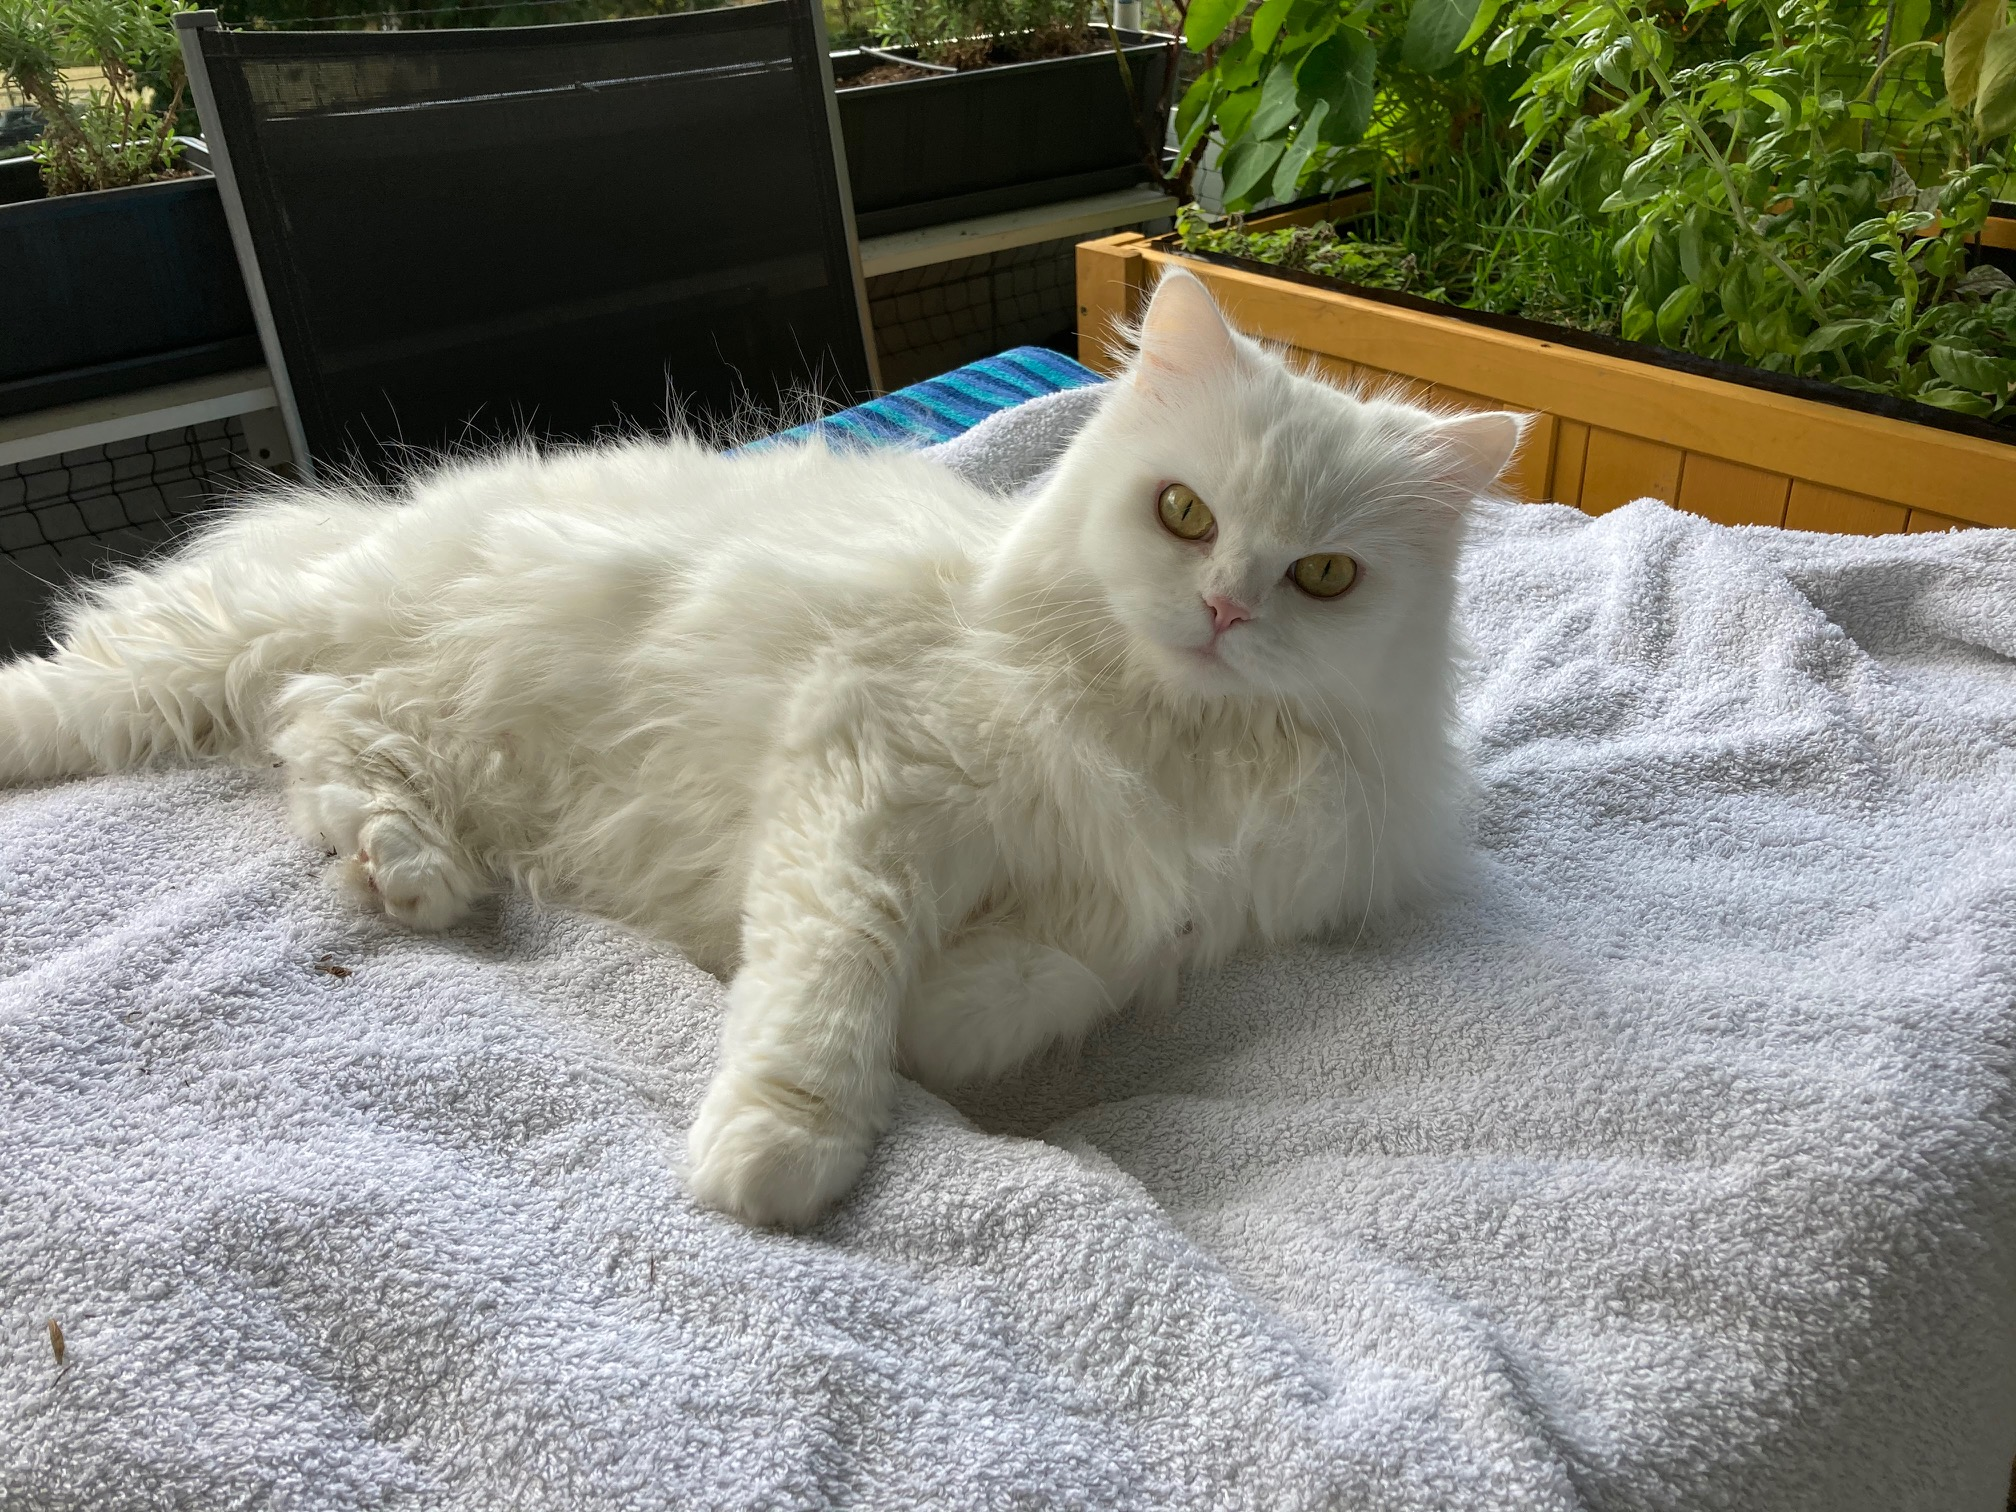
\includegraphics[width=\textwidth]{./Bilder/Katze1.jpg}
\caption{Meine Katze}
\end{figure}

\chapter{Mathematik}

Hallo, ich bin eine Formel \(a^2+b^2=c^2\). Und ich bin eine abgesetzte Formel ohne Nummer:

\[ a^2+b^2=c^2\]


\[
\frac{
	\frac{1}{2} + \frac{3}{4}}
	{\frac{5}{6} + \frac{7}{8}}  \]
	

Hallo, ich bin eine Formel \(\int_{i=1}^{1000} i^2 \). Und ich bin eine abgesetzte Formel ohne Nummer:
	
\[ \int_{i=1}^{1000} i^2   \]
	
\[ \avg 1234 = 456 \]

\begin{eqnarray}
y &=& d \\
y &=& d^2 +e^2
\end{eqnarray}

\[
\begin{array}{lcr} 
y &=& d   f\\
y &=& d^2 +e^2
\end{array}
\]


\end{document}